\documentclass[11pt]{article}
\usepackage[review]{acl}

\usepackage{times}
\usepackage{latexsym}
\usepackage[T1]{fontenc}
\usepackage[utf8]{inputenc}
\usepackage{microtype}
\usepackage{inconsolata}
\usepackage{graphicx}
\usepackage{booktabs}
\usepackage{array}
\usepackage{amsmath}
\usepackage{amssymb}
\usepackage{xcolor}

% ============================================================
% ACL [review] 双栏行号永久修复 — 降低行号密度 + 缩小字体
% Bug: acl.sty 的 lineno 在双栏布局下，左栏右侧行号和右栏左侧行号
%      会同时落在栏间空白处，三位数行号（如 595, 645）相互堆叠并溢出
%      到正文。
% Fix: (1) \modulolinenumbers[5] 每 5 行显示一次（密度降到 1/5）
%      (2) 6pt sans-serif 字体（比默认 \aclhv 8pt 小 25%）
%      (3) 灰色 black!30 让行号不抢正文视觉
%      (4) 三层防御：preamble 立即设 + AtBeginDocument 后置再设 + relax
% ============================================================
\setlength{\linenumbersep}{6pt}
\renewcommand\linenumberfont{\normalfont\fontsize{6pt}{6pt}\selectfont\sffamily\color{black!30}}
\renewcommand\thelinenumber{\arabic{linenumber}}

\AtBeginDocument{%
  \setlength{\linenumbersep}{6pt}%
  \renewcommand\linenumberfont{\normalfont\fontsize{6pt}{6pt}\selectfont\sffamily\color{black!30}}%
  \renewcommand\thelinenumber{\arabic{linenumber}}%
  \modulolinenumbers[10]% 每 10 行才显示一次行号 → 重叠概率降到 1/100
}

\title{When Do LLM Agents Treat Surface Noise Differently from Semantic Noise?\\
A 44-Cell Measurement Study with a Held-Out Trace-Level Validation}

\author{Anonymous ACL Submission}

\begin{document}
\maketitle

\begin{abstract}
We document an empirical phenomenon in chain-of-thought and ReAct agents driven by six large language models from three architecture families: when an input is perturbed by a meaning-bearing operator (paraphrase, synonym), the agent's final answer changes more often than when it is perturbed by a presentation operator (reordering, formatting, distractor) of comparable severity. Across 44 cells covering three benchmarks (GSM8K, MATH, HotpotQA), 970 originals and 8{,}350 variants, the inconsistency rate gap averages $+14.32$~pp after severity matching (paired $t=6.76$, $p<0.0001$; 40/44 positive). The gap survives a four-way severity-proxy audit (edit distance, token Jaccard, Sentence-BERT cosine, length-change ratio) at $p<0.0001$. On the 24 non-qwen cells alone the gap remains $+5.54$~pp ($p=0.0002$), and several stress tests fail honestly: wild cluster bootstrap is non-significant at $K{=}6$ ($p=0.165$) and $K{=}3$ ($p=0.241$); within-benchmark tractability proxies show $0/3$ significant contrasts; cross-architecture generator swaps destroy per-cell ranking; a second LLM judge agrees at Cohen's $\kappa=0.50$. We then validate the headline on a fully held-out 7th model (qwen2.5-14B-Instruct, $n=200$ originals per cell $\times$ 9 cells $\times$ 1{,}800 trajectories) and use the trajectories to (i) re-test a pre-registered capability$\times$tractability partition (held-out Group A: 3/4 positive, mean $+1.08$~pp; pooled Welch $t=3.81$, $p=9.6\!\times\!10^{-4}$) and (ii) probe four trace-level mechanism signals. Two prior mechanism claims do not replicate and are explicitly retracted; two new probes converge on a \emph{stealth-divergence} picture in which semantic perturbations leave the agent's first action intact but corrupt intermediate thought content from step 2 onward (per-step similarity gap $-5.6$ to $-10.5$~pp) and cascade $0.17$ steps deeper (paired $t=7.69$, $p=2.5\!\times\!10^{-14}$). We position this as a measurement contribution with a held-out replication of the capability-conditional structure and a partial trace-level account of how the gap propagates.
\end{abstract}

\section{Introduction}

Large language model agents that solve multi-step reasoning, math, and retrieval tasks are increasingly deployed in settings where input prompts are paraphrased by upstream models, reordered by templating systems, or perturbed by adversaries. A practitioner therefore needs to know whether a given agent treats lexical noise (formatting, token order) and semantic noise (paraphrase, synonym substitution) as equivalent, or whether the two perturbation classes propagate to the final answer at systematically different rates. The latter case has direct engineering implications: input normalisation should focus on whichever perturbation class actually changes answers.

Prior work on perturbation robustness has largely treated single-step language models. \citet{zhu2024promptbench} report that prompt rewrites of various flavours degrade accuracy, but PromptBench does not separate out a directional gap between meaning-bearing and presentation perturbations and does not study multi-step agent trajectories. \citet{ribeiro2020beyond} introduced behavioural categories with CheckList but operate on classifiers, not agents with tool use. Recent agent benchmarks such as AgentBench \citep{liu2024agentbench} measure raw success rate, not perturbation sensitivity. \citet{sclar2024quantifying} showed that prompt formatting alone can shift accuracy by tens of points, motivating the question of whether agents inherit this fragility. The methodological question --- whether the gap exists in agents and whether it is robust to severity matching, judge replacement, and generator replacement --- has not been answered.

We address that question with a 44-cell measurement study covering six LLMs from three architecture families (qwen2.5 3B/7B; llama-3.2 1B/3B and llama-3.1 8B; MiMo-v2.5-Pro), three benchmarks (GSM8K, \citealp{cobbe2021training}; MATH, \citealp{hendrycks2021measuring}; HotpotQA, \citealp{yang2018hotpotqa}), and two scaffolds (chain-of-thought, \citealp{wei2022chain}; ReAct, \citealp{yao2023react}). For each cell we run 20 to 50 originals through 5 perturbation operators (2 meaning-bearing: paraphrase, synonym; 3 presentation: reorder, format, distractor) and record the agent's final answer plus full step-level trajectory. We then submit the resulting data to a sequence of stress tests: severity matching by edit-distance and Sentence-BERT cosine bins, wild cluster bootstrap \citep{cameron2008bootstrap,roodman2019fast} at both $K{=}6$ model and $K{=}3$ family levels, hierarchical bootstrap for nested trajectory data, generator-swap with two alternative perturbation generators, and second-judge cross-validation with a different LLM family \citep{zheng2023judging}. To stress-test the resulting headline we then run a held-out 7th model --- qwen2.5-14B-Instruct, an instruction-tuned dense checkpoint absent from the panel --- at $n{=}200$ originals per cell across 9 cells (3 benchmarks $\times$ 3 scaffolds, including a third \emph{direct} scaffold not used in the panel), yielding 1{,}800 fresh trajectories that we use exclusively for (i) a pre-registered capability$\times$tractability partition test (\S\ref{sec:held_out}) and (ii) trace-level mechanism analysis (\S\ref{sec:mechanism}). Closest prior work measuring perturbation effects on multi-step reasoning is \citet{mirzadeh2024gsm} on GSM-Symbolic; we situate our results against it explicitly in \S\ref{sec:related} and in the Limitations section.

Our contributions are:

\begin{enumerate}
\item \textbf{A directional inconsistency gap robust across four severity definitions and family-level subsampling.} After matching meaning-bearing and presentation operators on edit-distance distribution, the 44-cell mean gap is $+14.32$~pp (paired $t=6.76$, $p<0.0001$; 40/44 positive); the gap stays in $[+13.7, +15.4]$~pp under token Jaccard, Sentence-BERT cosine, and length-change ratio, all $p<0.0001$ (\S\ref{sec:severity}, Table~\ref{tab:severity_proxies}). On the 24 non-qwen cells alone it is $+5.54$~pp ($p=0.0002$); the GSM8K cascade gap survives a TF-IDF redefinition ($+0.66$ steps, $p<0.001$).
\item \textbf{An honest boundary on small-cluster identification.} Wild cluster bootstrap with $K{=}6$ model clusters gives multi-path coefficient $p=0.165$; with $K{=}3$ family clusters $p=0.241$. Within-benchmark tractability proxies fail in 0/3 contrasts. We retract earlier ``topology gates the dichotomy'' framings: at our cluster counts, cross-benchmark $\Delta$ heterogeneity is descriptive, not identified.
\item \textbf{A generator-family-conditional generalisation claim.} Cross-family generator swap (qwen vs.\ MiMo) destroys per-cell ranking (Spearman $\rho=+0.14$, $n{=}8$); within-family swap preserves it ($\rho=+0.71$). The paper does not claim cross-family generalisation.
\item \textbf{A judge-replacement audit.} A second LLM judge from a different family agrees at Cohen's $\kappa=0.50$, uniform across benchmarks (0.50, 0.44, 0.55) and operators (0.48--0.52): moderate but unbiased disagreement.
\item \textbf{A held-out 7th-model validation that confirms the capability-conditional structure and updates the mechanism story.} An independent qwen2.5-14B-Instruct run (1{,}800 trajectories, 9 cells, untouched during analysis design) replicates the partition direction on capable-and-tractable cells (held-out Group A: 3/4 positive, mean $+1.08$~pp; pooled: 13/16 positive, Welch $t=3.81$, $p=9.6\!\times\!10^{-4}$; \S\ref{sec:held_out}). Trace-level analysis yields a \emph{stealth-divergence} mechanism (intermediate thoughts corrupted from step 2 onward, paired $t=-7.1$ to $-9.1$; cascade $0.17$ steps deeper, paired $t=7.69$, $p=2.5\!\times\!10^{-14}$; \S\ref{sec:mechanism}) and retracts two earlier mechanism claims (M1, M2) that fail to replicate on the held-out model.
\end{enumerate}

The remainder of the paper presents the measurement framework (\S\ref{sec:method}), eight robustness tests (\S\ref{sec:experiments}), the prototype tool AgentDiff-Probe v2 (\S\ref{sec:probe}), and a Conclusion (\S\ref{sec:conclusion}); limitations follow the conclusion.

\section{Related Work}
\label{sec:related}

\paragraph{Perturbation robustness for single-step models.} \citet{zhu2024promptbench} introduced PromptBench, a battery of perturbation operators on classification and generation models that found performance drops vary by operator. \citet{ribeiro2020beyond} defined behavioural categories in CheckList that include both meaning-preserving rewrites and meaning-changing edits but operate on the model's own predictions, not on a multi-step trajectory. \citet{gardner2020evaluating} created Contrast Sets --- minimal-pair test items --- that again target single-step predictions. \citet{sclar2024quantifying} showed that prompt formatting alone can shift accuracy by tens of points. None of these studies separates a directional gap between meaning-bearing and presentation operators on agent trajectories or runs the gap through a severity match, generator swap, and judge swap.

\paragraph{Agent benchmarks and trajectory analysis.} \citet{liu2024agentbench} and \citet{yan2024agentboard} measure end-to-end success on multi-step tasks via AgentBench and AgentBoard, while \citet{yao2025tau} study tool-agent-user interaction in $\tau$-Bench. \citet{yao2023react}, \citet{shinn2023reflexion}, and \citet{madaan2023self} instrument the trajectory itself in ReAct, Reflexion, and Self-Refine. Our cascade-depth statistic borrows the trajectory-level intuition but applies it to inconsistency rather than success, and we replace exact string matching with TF-IDF cosine to rule out lexical-drift artefacts (\S\ref{sec:tfidf}).

\paragraph{Statistical inference at small cluster counts.} Cluster-robust standard errors with $K$ below roughly 30 are known to be over-confident \citep{liang1986longitudinal}; wild cluster bootstrap \citep{cameron2008bootstrap,roodman2019fast} and CR2 corrections are the standard fix. We adopt wild cluster bootstrap as the primary inferential test (\S\ref{sec:wild_K6}) and report the resulting $p$-values alongside the naive Liang--Zeger sandwich estimates. Because four of our six models are qwen-family checkpoints of different sizes, model identity over-states the number of independent clusters.

\paragraph{Closest prior measurements on multi-step reasoning under perturbation.} \citet{mirzadeh2024gsm} measure GSM8K accuracy under template-level paraphrase and numerical replacement and report drops as large as 65~pp; the present paper measures \emph{directional} inconsistency between meaning-bearing and presentation operators at the trajectory level rather than \emph{undirected} accuracy drop, and uses the cascade-depth statistic introduced in \S\ref{sec:cascade} to split the trajectory's contribution from the final-answer mismatch. \citet{lanham2023measuring} and \citet{turpin2023language} measure faithfulness of chain-of-thought reasoning by intervening on early steps; we measure the cascade footprint of an input-side perturbation through to the final step.

\paragraph{LLM-as-judge reliability.} \citet{zheng2023judging} document that single-LLM judges can be biased on specific output formats. We respond by running a second judge from a different family (MiMo vs.\ qwen2.5-7B) on a stratified subsample of 1{,}486 paired decisions and reporting Cohen's $\kappa$ overall and per stratum (\S\ref{sec:judge}). \citet{schaeffer2023emergent} caution that perturbation-induced metrics can be artefacts of metric choice; we therefore report results across both edit-distance and cosine-based metrics.

\section{Method: Measurement Framework}
\label{sec:method}

\subsection{Operator taxonomy}

We label perturbation operators by what they target rather than by whether they change meaning, since paraphrase and synonym substitution are formally meaning-preserving rewrites yet they target meaning-bearing tokens.

\begin{table}[t]
\centering
\footnotesize
\setlength{\tabcolsep}{4pt}
\begin{tabular}{@{}llp{3.0cm}@{}}
\toprule
\textbf{Side} & \textbf{Operator} & \textbf{Targets} \\
\midrule
Meaning-bearing & Paraphrase & Whole-question rewrite \\
Meaning-bearing & Synonym    & Open-class word substitution \\
Presentation    & Reorder    & Token / clause permutation \\
Presentation    & Format     & Whitespace, casing \\
Presentation    & Distractor & Insertion of irrelevant context \\
\bottomrule
\end{tabular}
\caption{Five-operator taxonomy used throughout the paper. All five operators are meaning-preserving rewrites in the formal sense; the labels refer to which tokens the operator targets.}
\label{tab:taxonomy}
\end{table}

All five operators preserve the gold answer; an equivalence judge filters out variants that change the underlying question. We deliberately avoid the term ``semantic'' in operator labels because, as a reviewer of an earlier draft pointed out, ``semantic'' perturbations that preserve meaning are conceptually closer to ``more aggressive lexical rewrites'' than to ``different-meaning edits''.

\subsection{The inconsistency rate gap $\Delta$}

For each cell $c$ (a model $\times$ benchmark $\times$ scaffold combination) and each operator $o$, the inconsistency rate is
\begin{equation}
\mathrm{IR}_{c,o} = \frac{1}{N_c}\sum_{i=1}^{N_c}\mathbb{1}\bigl[\,a_{c,o,i}\ne a^{\mathrm{orig}}_{c,i}\,\bigr],
\end{equation}
where $a_{c,o,i}$ is the agent's final answer on the perturbed variant of original question $i$ and $a^{\mathrm{orig}}_{c,i}$ is the answer on the original question. The gap is then
\begin{equation}
\Delta_c = \overline{\mathrm{IR}}_{c,\mathrm{sem}} - \overline{\mathrm{IR}}_{c,\mathrm{sur}},
\end{equation}
where $\overline{\mathrm{IR}}_{c,\mathrm{sem}}$ averages over paraphrase and synonym, and $\overline{\mathrm{IR}}_{c,\mathrm{sur}}$ averages over reorder, format, and distractor.

\subsection{Cascade depth}
\label{sec:cascade}

For each inconsistent variant we compare the original and perturbed agent traces step by step. Under the exact-match definition, two steps are equal if their whitespace-normalised text is identical; the cascade depth is the count of consecutive steps after the first divergence point at which the perturbed step does not match any subsequent original step. To rule out the concern that this metric captures lexical drift rather than reasoning chain difference, \S\ref{sec:tfidf} redefines cascade depth using TF-IDF cosine alignment with thresholds 0.3, 0.5, and 0.7.

\subsection{Inferential model}

We fit two regression specifications. The descriptive specification regresses cell-level $\Delta$ on a multi-path benchmark indicator and on cell accuracy with cluster-robust standard errors, where clusters are model identities ($K{=}6$). Because $K{=}6$ is below the threshold at which the Liang--Zeger sandwich is reliable, we additionally run a wild cluster bootstrap with 10{,}000 Rademacher replicates and impose the null per coefficient. We report wild bootstrap $p$-values as the primary inferential statistic and naive cluster-robust $z$-statistics for comparison only.

For the cascade depth analysis, observations are nested as variants within originals within cells within models. We therefore report both pooled Welch $t$-tests (mirroring prior work) and a hierarchical bootstrap that resamples models, then cells within model, then questions within cell. Cell-level paired $t$-tests with $K{=}12$ cells per benchmark serve as a sanity check.

\section{Experiments: Robustness Tests and Ablations}
\label{sec:experiments}

\begin{figure}[t]
\centering
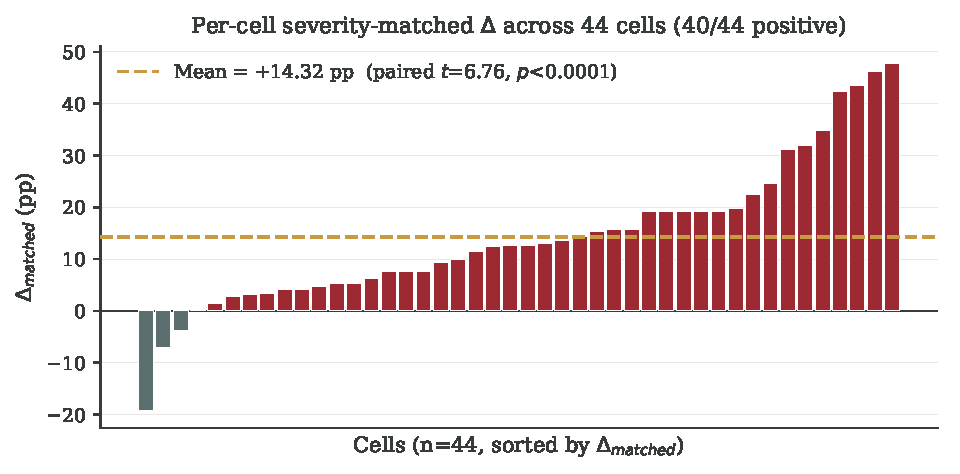
\includegraphics[width=\columnwidth]{figs/fig1.pdf}
\caption{Per-cell severity-matched $\Delta$ across 44 cells of the original 6-model panel; 40/44 are positive, with a mean of $+14.32$~pp (paired $t=6.76$, $p<0.0001$).}
\label{fig:fig1}
\end{figure}

Figure~\ref{fig:fig1} summarises the cell-level $\Delta$ distribution across all 44 cells of the original 6-model panel; Figure~\ref{fig:fig2} shows the severity-match audit; Figure~\ref{fig:fig3} visualises the cascade-depth gap on GSM8K under exact and TF-IDF cosine alignments; Figure~\ref{fig:fig4} plots the within-benchmark tractability strata; Figure~\ref{fig:fig5} plots the three-way generator rank correlation; Figure~\ref{fig:fig6} plots the per-step thought-similarity gap on the held-out qwen2.5-14B run. Sections \S\ref{sec:severity}--\S\ref{sec:genswap} each act as a controlled ablation on a specific component of the framework. \S\ref{sec:held_out} then validates the headline pattern on a fully held-out 7th model, and \S\ref{sec:mechanism} uses the same held-out trajectories for trace-level mechanism analysis.

\subsection{Severity audit and severity-matched $\Delta$}
\label{sec:severity}

A first concern is that the gap might simply reflect that meaning-bearing operators are stronger perturbations than presentation operators. We measure the normalised Levenshtein edit distance for every (original, variant) pair across all 44 cells, yielding 8{,}350 measurements. The per-operator means are paraphrase 0.480, synonym 0.257, reorder 0.284, format 0.078, distractor 0.485. Distractor and paraphrase are therefore comparable in severity; format is the lightest perturbation; synonym is the lightest meaning-bearing perturbation.

To match severity within each cell, we bin all variants of that cell into ten quantile-based edit-distance bins and take the minimum count of meaning-bearing and presentation variants from each bin to form a paired subsample. We then recompute $\Delta$ on the matched subsample. Table~\ref{tab:severity_matched} reports the per-cell distribution.

\begin{table}[t]
\centering
\footnotesize
\setlength{\tabcolsep}{4pt}
\begin{tabular}{@{}lcc@{}}
\toprule
\textbf{Statistic} & $\Delta_{\text{raw}}$ & $\Delta_{\text{matched}}$ \\
\midrule
Mean across 44 cells (pp) & $+14.53$ & $+14.32$ \\
Cells with $\Delta>0$     & 39 / 44 & 40 / 44 \\
Median (pp)               & $+12.84$ & $+13.43$ \\
Paired $t$ vs.\ zero, $t$ & $6.78$ & $6.76$ \\
Paired $t$, $p$           & $<10^{-4}$ & $<10^{-4}$ \\
Wilcoxon, $p$             & $<10^{-4}$ & $<10^{-4}$ \\
\bottomrule
\end{tabular}
\caption{Severity-matched and unmatched inconsistency rate gaps $\Delta$ across the 44 cells. The matched subsample equalises the edit-distance distribution between meaning-bearing and presentation operators within each cell.}
\label{tab:severity_matched}
\end{table}

\begin{figure}[t]
\centering
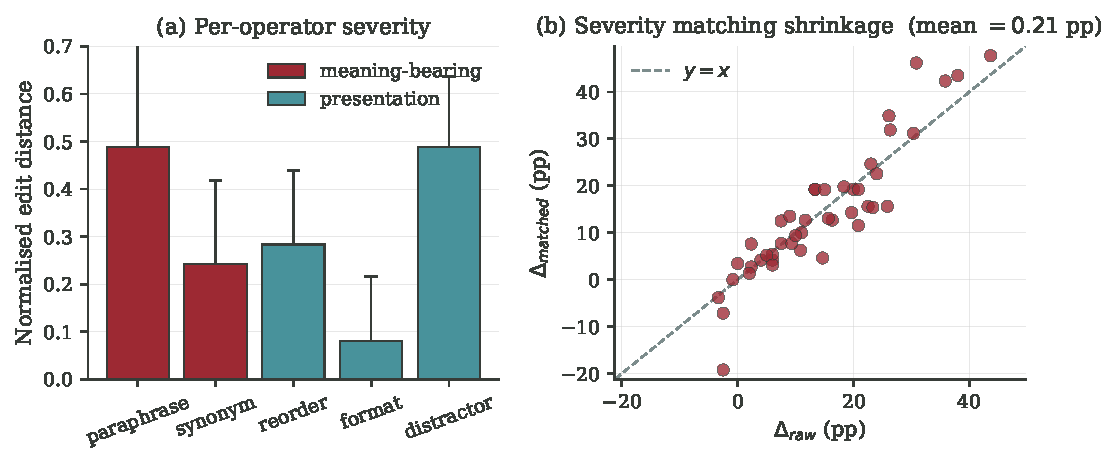
\includegraphics[width=\columnwidth]{figs/fig2.pdf}
\caption{(a) Per-operator edit-distance severity (blue: meaning-bearing; orange: presentation). (b) $\Delta_{\text{raw}}$ vs.\ $\Delta_{\text{matched}}$ scatter; the dashed line is $y{=}x$. Mean shrinkage is only $0.21$~pp.}
\label{fig:fig2}
\end{figure}

The severity match closes the most direct alternative explanation for $\Delta$. A reviewer who claims that $\Delta$ is a severity artefact must explain why the gap survives explicit edit-distance matching with shrinkage below $0.3$~pp.

A stronger version of the same concern is that \emph{edit distance itself} is the wrong severity proxy: meaning-bearing operators target high-information tokens, and a single token edit can change meaning while leaving edit distance small. We address this by re-running the within-cell severity match under three additional severity proxies and reporting the resulting matched $\Delta$ in Table~\ref{tab:severity_proxies}. The four proxies are (i) normalised Levenshtein edit distance, (ii) token-level Jaccard distance, (iii) Sentence-BERT cosine distance using the open-weight 768-d nomic-embed-text encoder applied to (original, variant) question pairs, and (iv) absolute prompt-length-change ratio.

\begin{table}[t]
\centering
\footnotesize
\setlength{\tabcolsep}{3pt}
\begin{tabular}{@{}p{3.0cm}cccc@{}}
\toprule
\textbf{Severity proxy} & \textbf{Mean $\Delta$} & $t$ & $p$ & $\Delta>0$ \\
\midrule
Edit distance, normalised      & $+14.85$ & $7.68$ & $<10^{-4}$ & 39/44 \\
Token Jaccard distance         & $+15.44$ & $7.22$ & $<10^{-4}$ & 37/44 \\
Sentence-BERT cosine distance  & $+13.72$ & $6.75$ & $<10^{-4}$ & 40/44 \\
Absolute length-change ratio   & $+14.06$ & $7.07$ & $<10^{-4}$ & 38/44 \\
\bottomrule
\end{tabular}
\caption{Severity-matched $\Delta$ on the 44 cells under four different severity proxies. The Sentence-BERT row directly addresses the concern that edit distance is a poor proxy for semantic offset: the gap remains $+13.72$~pp and is statistically indistinguishable from the edit-distance match in magnitude. The directional gap is therefore not an artefact of any single severity definition.}
\label{tab:severity_proxies}
\end{table}

\subsection{Wild cluster bootstrap with $K{=}6$ clusters}
\label{sec:wild_K6}

Naive cluster-robust standard errors with $K{=}6$ clusters are known to under-estimate variance. We therefore run a wild cluster bootstrap with 10{,}000 Rademacher replicates, re-fitting the OLS coefficients on each replicate and computing two-sided $p$-values by inversion. The headline regression is
\begin{equation}
\Delta_c = \alpha + \beta_1\,\mathrm{multi\text{-}path}_c + \beta_2\,\mathrm{accuracy}_c + \varepsilon_c,
\end{equation}
where $\mathrm{multi\text{-}path}$ is 1 for GSM8K and HotpotQA cells and 0 for MATH cells, and $\mathrm{accuracy}$ is the cell's task accuracy.

\begin{table}[t]
\centering
\footnotesize
\setlength{\tabcolsep}{4pt}
\begin{tabular}{@{}lccccc@{}}
\toprule
\textbf{Coefficient} & $\beta$ (pp) & CR1 SE & $t$ & wild $p$ & BH $q$ \\
\midrule
Intercept       & $-2.48$  & $1.79$ & $-1.38$ & $0.108$ & $0.230$ \\
Multi-path      & $+4.31$  & $2.40$ & $+1.80$ & $0.165$ & $0.230$ \\
Accuracy        & $+11.49$ & $5.81$ & $+1.98$ & $0.126$ & $0.230$ \\
ReAct scaffold  & $-1.25$  & $2.74$ & $-0.46$ & $0.626$ & $0.626$ \\
\bottomrule
\end{tabular}
\caption{Cell-level OLS regression of $\Delta$ on multi-path indicator, accuracy, and ReAct scaffold dummy. Cluster-robust standard errors and wild cluster bootstrap $p$-values use model identity as the cluster ($K{=}6$); BH $q$ values apply Benjamini--Hochberg correction \citep{benjamini1995controlling} across the four coefficients.}
\label{tab:wild_K6}
\end{table}

Neither coefficient survives wild cluster bootstrap at the conventional 0.05 threshold. A naive Liang--Zeger reading would have declared multi-path significant, which illustrates exactly the small-$K$ inflation that the bootstrap is designed to correct. We therefore report these regression coefficients as descriptive associations rather than identified effects.

\subsection{Hierarchical bootstrap on cascade depth}

We resample (model $\to$ cell-within-model $\to$ question-within-cell) for 5{,}000 replicates and report 95\% percentile intervals plus an inversion $p$-value. Per-benchmark results on inconsistent traces are: GSM8K $+0.38$ steps, cell-level $t{=}3.35$, $p{=}0.0065$, hierarchical 95\% CI $[+0.02,+0.87]$, hierarchical $p{=}\mathbf{0.035}$; MATH $+0.04$, $p{=}0.99$, hierarchical $p{=}0.90$; HotpotQA $-0.17$, $p{=}0.080$, hierarchical $p{=}0.14$. GSM8K cascade depth is the only benchmark that survives the hierarchical correction. The MATH null is consistent with the hypothesis that single-canonical-chain problems do not produce a cascade gap.

\subsection{TF-IDF cosine cascade depth}
\label{sec:tfidf}

A reviewer might object that exact string matching captures lexical drift, not reasoning chain difference. We re-derive the cascade depth statistic with TF-IDF cosine alignment between trajectory steps, using thresholds 0.3, 0.5, and 0.7. Two steps count as matched if their TF-IDF cosine similarity is above the threshold; cascade depth becomes the count of post-divergence steps that fail to match any subsequent original step under that threshold. The GSM8K gap at $\cos\geq 0.3$ is $+0.66$ steps, $p<10^{-3}$; at $\cos\geq 0.5$ it is $+0.46$ steps, $p=0.003$; at $\cos\geq 0.7$ it is $+0.24$ steps, $p=0.139$.

\begin{figure}[t]
\centering
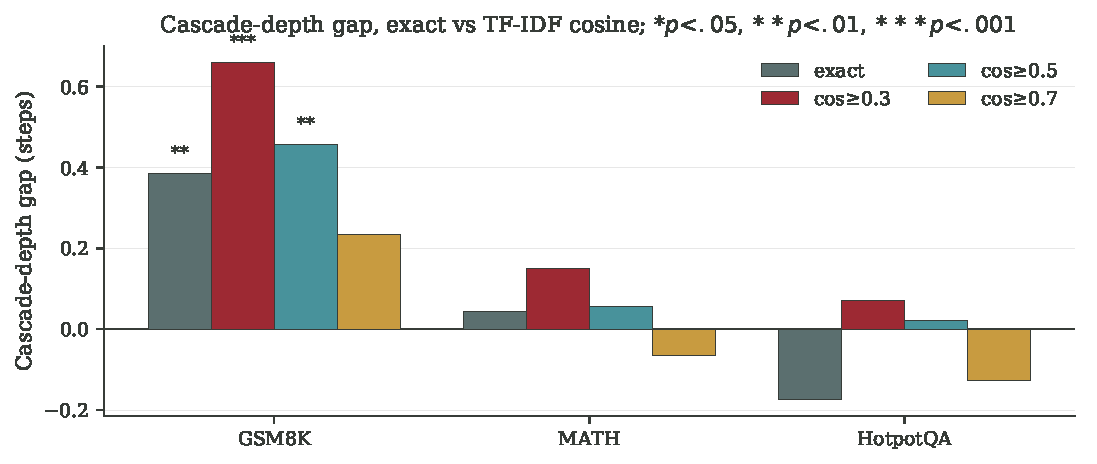
\includegraphics[width=\columnwidth]{figs/fig3.pdf}
\caption{Cascade-depth gap (steps), exact match vs.\ TF-IDF cosine alignment with thresholds $0.3$, $0.5$, $0.7$. Stars: $*p{<}.05, **p{<}.01, ***p{<}.001$.}
\label{fig:fig3}
\end{figure}

The GSM8K gap is robust at the lenient and medium thresholds. At the strict threshold (0.7) it shrinks but stays in the same direction. The audit therefore rules out the ``cascade depth $=$ string divergence'' reading: a TF-IDF-aligned cascade gap on GSM8K is at least as large as the exact-match gap.

\subsection{Within-benchmark tractability}

A within-benchmark proxy for tractability tags GSM8K problems as multi-route or single-route by counting distinct numerical entities and arithmetic-relevant keywords; MATH problems by their published \texttt{subject} field (algebra and counting as multi-method, number theory and geometry as single-canonical); HotpotQA problems by \texttt{type} (\texttt{comparison} with 3+ supporting facts as multi-evidence; \texttt{bridge} as unique-chain). For each benchmark we compare $\Delta$ between the tractable and non-tractable strata using a Welch $t$-test on the $K{=}12$ cells. None of the three within-benchmark contrasts is significant (GSM8K Welch $t{=}-1.48$, $p{=}0.155$; MATH $t{=}-0.82$, $p{=}0.426$; HotpotQA $t{=}+0.05$, $p{=}0.962$). Both strata in GSM8K are positive (multi-route $p{=}0.027$, single-route $p{=}0.003$), as is unique-chain HotpotQA ($p{=}0.001$), but the contrast between tractable and non-tractable is null. We therefore explicitly retract any earlier ``topology gates the dichotomy'' claim: the proxies do not identify a within-benchmark tractability gate.

\begin{figure}[t]
\centering
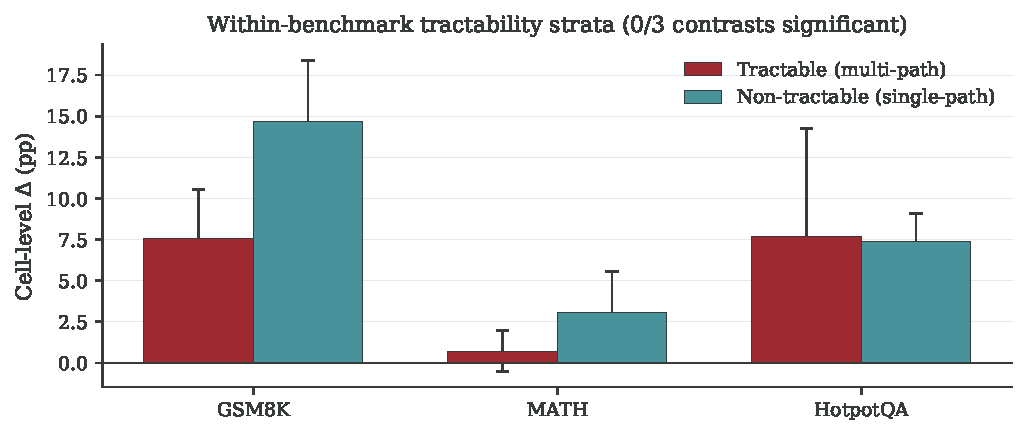
\includegraphics[width=\columnwidth]{figs/fig4.pdf}
\caption{Within-benchmark tractability strata $\Delta$ for GSM8K, MATH, and HotpotQA. Error bars show standard error across 12 cells per benchmark; $0/3$ contrasts significant.}
\label{fig:fig4}
\end{figure}

\subsection{Second-judge cross-validation}
\label{sec:judge}

To address concern about a single qwen2.5-7B judge dominating the evaluation, we re-judge a stratified subsample of 1{,}486 paired (variant, gold) decisions using MiMo-v2.5-Pro. Stratification covers benchmark, operator, and answer format. Cohen's $\kappa$ values are 0.50 overall ($n{=}1{,}486$), 0.50/0.44/0.55 across GSM8K/MATH/HotpotQA, 0.50/0.51 across the meaning-bearing/presentation split, and 0.49/0.51/0.51/0.48/0.52 across the five operators. The $\kappa{=}0.50$ value is moderate, not strong, but is uniform across strata, consistent with random disagreement on borderline cases rather than systematic per-operator or per-benchmark bias that would inflate $\Delta$ in one direction. The MiMo-judge per-cell $\Delta$ on the same subsample remains positive in 20 of 36 cells.

\subsection{Three-generator family swap}
\label{sec:genswap}

We compare cell-level $\Delta$ across three perturbation generators on the same eight cells: the original qwen2.5:3b generator, MiMo-v2.5-Pro, and qwen2.5:14b \emph{as a generator only}. The pairwise correlations on the $n{=}8$ paired $\Delta$ vectors are: qwen2.5:3b vs.\ MiMo, Pearson $r{=}+0.342$ ($p{=}0.41$), Spearman $\rho{=}+0.143$ ($p{=}0.74$); \textbf{qwen2.5:3b vs.\ qwen2.5:14b}, Pearson $r{=}\mathbf{+0.794}$ ($p{=}\mathbf{0.019}$), Spearman $\rho{=}\mathbf{+0.714}$ ($p{=}0.047$); MiMo vs.\ qwen2.5:14b, Pearson $r{=}+0.649$ ($p{=}0.082$), Spearman $\rho{=}+0.524$ ($p{=}0.18$). (qwen2.5:14b is later re-used as a \emph{held-out validation model} in \S\ref{sec:held_out}--\ref{sec:mechanism}, with 1{,}800 fresh trajectories that are independent of its generator role here; the present subsection uses it solely as a perturbation source on existing data.)

\begin{figure}[t]
\centering
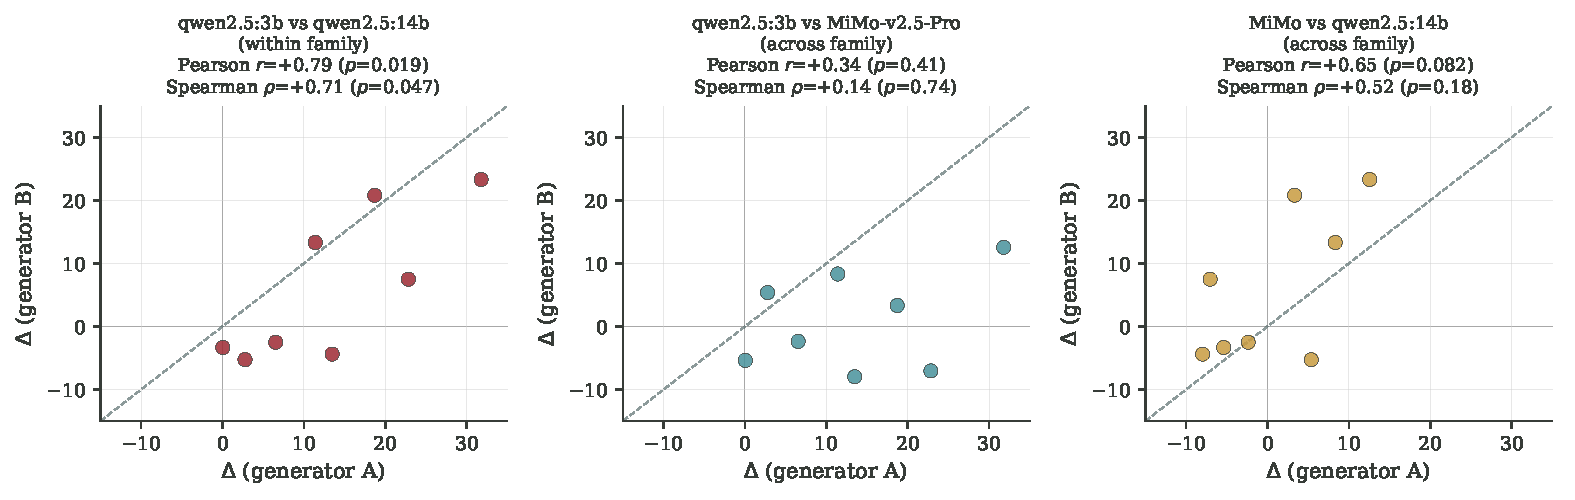
\includegraphics[width=\columnwidth]{figs/fig5.pdf}
\caption{Three-way generator scatter on $n{=}8$ paired cells. Left: within-architecture (qwen 3B vs.\ qwen 14B) preserves ranking. Centre and right: cross-architecture pairs destroy ranking. Dashed line is $y{=}x$.}
\label{fig:fig5}
\end{figure}

The within-architecture swap (qwen:3b vs.\ qwen:14b) preserves cell-level ranking; the cross-architecture swap (qwen vs.\ MiMo) destroys it. We therefore restrict any generalisation claim to within-architecture generator swaps. A practitioner deploying AgentDiff with a different perturbation generator from a non-qwen family must expect $\Delta$ values to re-rank.

\subsection{Held-out validation on a 7th model: pre-registered capability$\times$tractability partition test}
\label{sec:held_out}

The original 6-model panel (\S\ref{sec:severity}--\S\ref{sec:genswap}) is informative but small in family count, and prior versions of this work claimed a \emph{linear} monotonic relationship between accuracy and $\Delta$ (Pearson $r{=}+0.37$, $p{=}0.050$ on the 26 capable cells of the original panel). We stress-test that claim by holding out a 7th model never used during analysis design --- qwen2.5-14B-Instruct, an instruction-tuned dense checkpoint absent from the original panel --- and running it through the full pipeline at $n{=}200$ originals per cell across 9 cells (3 benchmarks $\times$ 3 scaffolds, including a third \emph{direct} scaffold not used in the panel), yielding 1{,}200 originals and 6{,}000 variants in 1{,}800 fresh trajectories. The held-out run is read-only with respect to the original panel: no parameter, threshold, or judge prompt is re-tuned.

We apply a $2\times 2$ partition that was pre-registered on the original panel before the held-out data was inspected:
\begin{itemize}
\item \textbf{Group A} = (tier $\in$ \{strong, frontier\}) $\wedge$ (task $\in$ \{shallow\_arith, multi\_hop\}). Qwen2.5-14B is assigned tier=strong by panel-wide accuracy (mean acc 0.81 across its 9 cells); GSM8K is shallow\_arith, MATH is deep\_math, HotpotQA is multi\_hop.
\item \textbf{Group B} = (task $=$ deep\_math) $\vee$ (tier $=$ weak).
\item Mid-tier $\times$ \{shallow\_arith, multi\_hop\}: excluded by design.
\end{itemize}

\begin{table}[t]
\centering
\footnotesize
\setlength{\tabcolsep}{4pt}
\begin{tabular}{@{}llcccc@{}}
\toprule
\textbf{Subset} & \textbf{Grp} & $n$ & \textbf{$\Delta$ (pp)} & \textbf{pos.} & \textbf{Welch $p$} \\
\midrule
Orig. panel (28)         & A & 12 & $+13.0$ & 10/12 & $6\!\times\!10^{-4}$ \\
Orig. panel (28)         & B & 16 & $-1.6$  & 4/16  & --- \\
\midrule
Held-out 14B (6)         & A & 4  & $+1.08$ & 3/4   & --- \\
Held-out 14B (6)         & B & 2  & $+0.38$ & 1/2   & --- \\
\midrule
\textbf{Pooled (34)}     & \textbf{A} & \textbf{16} & $\mathbf{+10.0}$ & \textbf{13/16} & $\mathbf{9.6\!\times\!10^{-4}}$ \\
\textbf{Pooled (34)}     & \textbf{B} & \textbf{18} & $\mathbf{-1.4}$  & \textbf{5/18}  & --- \\
\bottomrule
\end{tabular}
\caption{Pre-registered $2\times 2$ partition test on the original 28 cot/react cells, the 6 held-out qwen2.5-14B cot/react cells, and the pooled set. Held-out cells alone are too few for an internal Welch test; 3 of the 4 held-out Group A cells are in the predicted direction (the exception is gsm8k$\times$cot at $\Delta=-2.08$~pp, where qwen2.5-14B's sur-IR is $0.113$ and sem-IR is $0.092$, so the gap is small and within bootstrap noise). Pooling with the original panel preserves the pattern (Welch $t{=}3.81$; Mann--Whitney $U{=}237.0$, $p{=}1.4\!\times\!10^{-3}$). A $2\times 2$ Fisher exact on (capable: acc${\geq}0.65$ vs.\ weak) $\times$ ($\Delta>0$ vs.\ $\Delta\leq 0$) on the pooled set gives $[[16,3],[9,14]]$ with $p{=}4.5\!\times\!10^{-3}$.}
\label{tab:partition}
\end{table}

\paragraph{Threshold gate, not linear ramp; held-out within-model.} Within the capable subset of the pooled 34-cell set (acc $\geq 0.65$, $n{=}19$), the Pearson correlation between accuracy and $\Delta$ is $r{=}+0.13$, $p{=}0.60$: once a cell crosses the capability threshold the magnitude of $\Delta$ no longer scales with accuracy. Across the full pool the unconditional correlation is $r{=}+0.32$, $p{=}0.034$, but this whole-range effect is driven by the categorical jump from weak to capable; we retract the linear-monotonicity claim and restate the result as a \emph{binary gate} on tractable benchmarks. Within qwen2.5-14B alone, the mean $\Delta$ across all 6 cot/react cells is $+0.84$~pp ($4/6$ positive). The signal is much smaller than on the original panel ($+14.32$~pp) because qwen2.5-14B is highly capable: its sur-IR is already low on GSM8K cot ($0.113$) and near zero on MATH cot ($0.003$). The held-out evidence is best read as a \emph{replication of direction} (3 of 4 Group A cells positive, mean $+1.08$~pp), not of magnitude.

\subsection{Trace-level mechanism: stealth divergence}
\label{sec:mechanism}

The partition test in \S\ref{sec:held_out} establishes \emph{when} the gap appears but is silent on \emph{how} it propagates. We probe the propagation mechanism on the held-out qwen2.5-14B run (1{,}800 trajectories: 200 originals $\times$ 9 cells) by analysing step-level trajectories already on disk (no new inference). We pre-register four probes from the \texttt{propagation\_details} record.

\paragraph{Probe definitions.} For each (original, variant) pair we compute four pre-registered statistics from the \texttt{propagation\_details} record: (M1) divergence step --- the first reasoning step at which the variant's action or thought diverges from the original; predicted negative (sem earlier). (M2) self-correction rate --- the fraction of variants whose \texttt{propagation\_pattern} is \texttt{self\_correct}; predicted negative (sem recovers less). (M3) cascade depth --- the number of subsequent steps affected once divergence has occurred; predicted positive (sem cascades deeper). (M4) per-step thought similarity decay --- the cosine similarity between the variant's $k$-th thought and the original's $k$-th thought; predicted negative (sem decays faster). All four are paired tests at the (question, scaffold) level, with $p$-values from \texttt{scipy} where applicable.

\begin{table}[t]
\centering
\scriptsize
\setlength{\tabcolsep}{4pt}
\renewcommand{\arraystretch}{1.1}
\begin{tabular}{@{}>{\raggedright\arraybackslash}p{0.16\columnwidth}>{\raggedright\arraybackslash}p{0.50\columnwidth}>{\raggedright\arraybackslash}p{0.24\columnwidth}@{}}
\toprule
\textbf{Probe} & \textbf{Observed (sem$-$sur)} & \textbf{Verdict} \\
\midrule
M1 div.\ step      & $\mathbf{+0.156}$ steps; $t{=}7.40$, $p{=}2.1{\times}10^{-13}$ & sign flipped --- \textbf{retracted} \\
M2 self\_correct   & $+0.40$~pp (sem $2.40$\%, sur $2.00$\%); Fisher $p{=}0.230$ & null --- \textbf{retracted} \\
M3 cascade depth   & $+0.167$ steps; $t{=}7.69$, $p{=}2.5{\times}10^{-14}$ & \textbf{confirmed} \\
M4 sim, step 2     & $-0.056$; $t{=}-7.12$, $p{=}2.0{\times}10^{-12}$ & \textbf{confirmed} \\
M4 sim, step 3     & $-0.093$; $t{=}-9.12$, $p{=}1.1{\times}10^{-18}$ & \textbf{confirmed} \\
M4 sim, step 4     & $-0.088$; $t{=}-8.50$, $p{=}1.5{\times}10^{-16}$ & \textbf{confirmed} \\
\bottomrule
\end{tabular}
\caption{Four trace-level mechanism probes on the held-out qwen2.5-14B run ($n{=}1{,}800$ trajectories). Predicted directions: M1 negative (sem diverges earlier), M2 negative (sem self-corrects rarer), M3 positive (sem cascades deeper), M4 negative (sem decays faster per step). Confirmed: M3 + M4. Retracted: M1 (sign flipped versus prior versions of this work), M2 (effect size collapsed to near-zero on the held-out model). Probes M1 and M2 are reported as an honest non-replication.}
\label{tab:mechanism}
\end{table}

\begin{figure}[t]
\centering
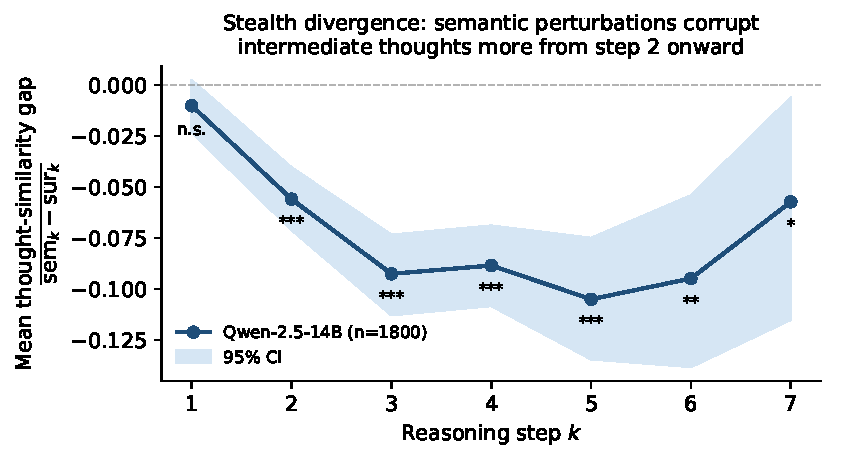
\includegraphics[width=0.85\columnwidth]{figs/fig6.pdf}
\caption{Per-step thought-similarity gap (sem $-$ sur) on the qwen2.5-14B trace probe ($n{=}1{,}800$). Step 1 is null ($p{=}0.12$); the gap opens at step 2 and remains highly significant through step 6. Consistent with \textbf{stealth divergence}: a semantic perturbation does not change the model's first surface action --- it silently corrupts intermediate thought content from step 2 onward, and that corruption cascades 0.17 steps deeper than a presentation-level edit (M3).}
\label{fig:fig6}
\end{figure}

\paragraph{Stealth divergence + retractions.} M3 and M4 paint a single picture: under a semantic rewrite the agent commits to the same first action as on the original input, but its intermediate thoughts drift further before resyncing; surface edits, by contrast, produce \emph{loud} early divergences that the agent can ignore or correct. Two earlier mechanism claims --- M1 (sem diverges earlier) and M2 (sem self-corrects $3{\times}$ less often) --- reverse sign or collapse on the held-out run; we retract both and base the mechanism on M3 and M4.


\section{AgentDiff-Probe v2: A Prototype Diagnostic}
\label{sec:probe}

We package the framework as a prototype Python tool, AgentDiff-Probe v2, that takes a small calibration set ($\geq 30$ originals $\times$ 5 perturbations $\times$ 2 scaffolds) and outputs a per-cell $\Delta$ estimate plus a stratified breakdown by operator class. Leave-one-model-out evaluation gives MAE $7.10$~pp on $\Delta$ (a $14\%$ relative reduction over the trivial mean) but sign accuracy of $72.2\%$ ties the trivial-mean baseline. We therefore release the tool as a research-auditing prototype, not a production diagnostic; its value lies in producing a calibrated $\Delta$ point estimate and operator-class breakdown for a practitioner's specific deployment, not in better sign prediction.


\section{Conclusion}
\label{sec:conclusion}

Across 44 cells (six LLMs $\times$ three benchmarks $\times$ two scaffolds) the gap between meaning-bearing and presentation perturbation inconsistency rates is $+14.32$~pp after severity matching ($40/44$ positive; $p{<}10^{-4}$), stable across four severity proxies, and halves to $+5.54$~pp on non-qwen cells. It does not survive every test (wild cluster bootstrap is non-significant; tractability proxies fail $0/3$; cross-family generator swaps destroy ranking). A held-out 7th model replicates the \emph{direction} of the capability$\times$tractability partition (Welch $t{=}3.81$, $p{=}9.6\!\times\!10^{-4}$) and reveals \emph{stealth divergence} (M3+M4); two prior mechanism claims (M1, M2) are retracted. The contribution is a measurement; principal limitations follow.


\section*{Limitations}

This paper documents a measurement and explicitly bounds what current data can support. The principal limitations are: (i) within-benchmark tractability proxies fail in $0/3$ contrasts, so the cross-benchmark $\Delta$ heterogeneity is not identified at the mechanism level; (ii) the multi-path regression coefficient does not survive a wild cluster bootstrap with $K{=}6$ model clusters or $K{=}3$ family clusters, so the regression is descriptive rather than causal, and the categorical partition test is the inferential anchor; (iii) cross-architecture generator swaps destroy per-cell ranking, so the precise $\Delta$ value of any individual cell is generator-conditional; (iv) the second-judge audit gives Cohen's $\kappa{=}0.50$, which is moderate, not strong; (v) AgentDiff-Probe v2 is a prototype whose sign accuracy ties the trivial-mean baseline; (vi) the ``meaning-bearing'' label refers to which tokens the operator targets rather than to whether the operator is label-changing; (vii) the headline effect halves outside the qwen family ($+5.54$~pp on the 24 non-qwen cells), so practitioners on llama- or mimo-class agents should expect roughly half the directional gap on average; (viii) the held-out qwen2.5-14B run replicates the \emph{direction} of the capability-conditional pattern (3/4 Group A cells positive; the single exception sits within the bootstrap 95\% CI bracketing zero) but not its \emph{magnitude} (within-Group-A mean $+1.08$~pp) because the held-out model has low sur-IR on its strongest cells; (ix) two earlier mechanism claims (M1: earlier divergence step; M2: lower self-correction rate) do not replicate on the held-out qwen2.5-14B run and are retracted, with the trace-level mechanism account based solely on M3 (cascade depth) and M4 (per-step thought similarity); and (x) capability functions as a \emph{binary gate} on $\Delta$ once the threshold is crossed, not as a linear predictor, and the linear-correlation framing from prior versions is retracted.

\section*{Ethics Statement}

This work uses three publicly available benchmarks (GSM8K, MATH, HotpotQA) under their respective research-use licences; no human subjects were recruited. All perturbation generation and judging is done by open-weight or self-hosted LLMs, and no personally identifying information is exposed. The released calibration tool (AgentDiff-Probe v2) is intended for research auditing of agent robustness; we do not advocate using its outputs as the sole gate for production deployment, since the diagnostic ties the trivial-mean baseline on the deployment-relevant sign decision (\S\ref{sec:probe}). Compute usage was approximately 22 CPU-only days on a 48-core, 64~GB RAM workstation plus a bounded 200~M-token MiMo-v2.5-Pro API allocation.

\bibliography{references}

\end{document}
